\section{Design}
\label{sec:design}

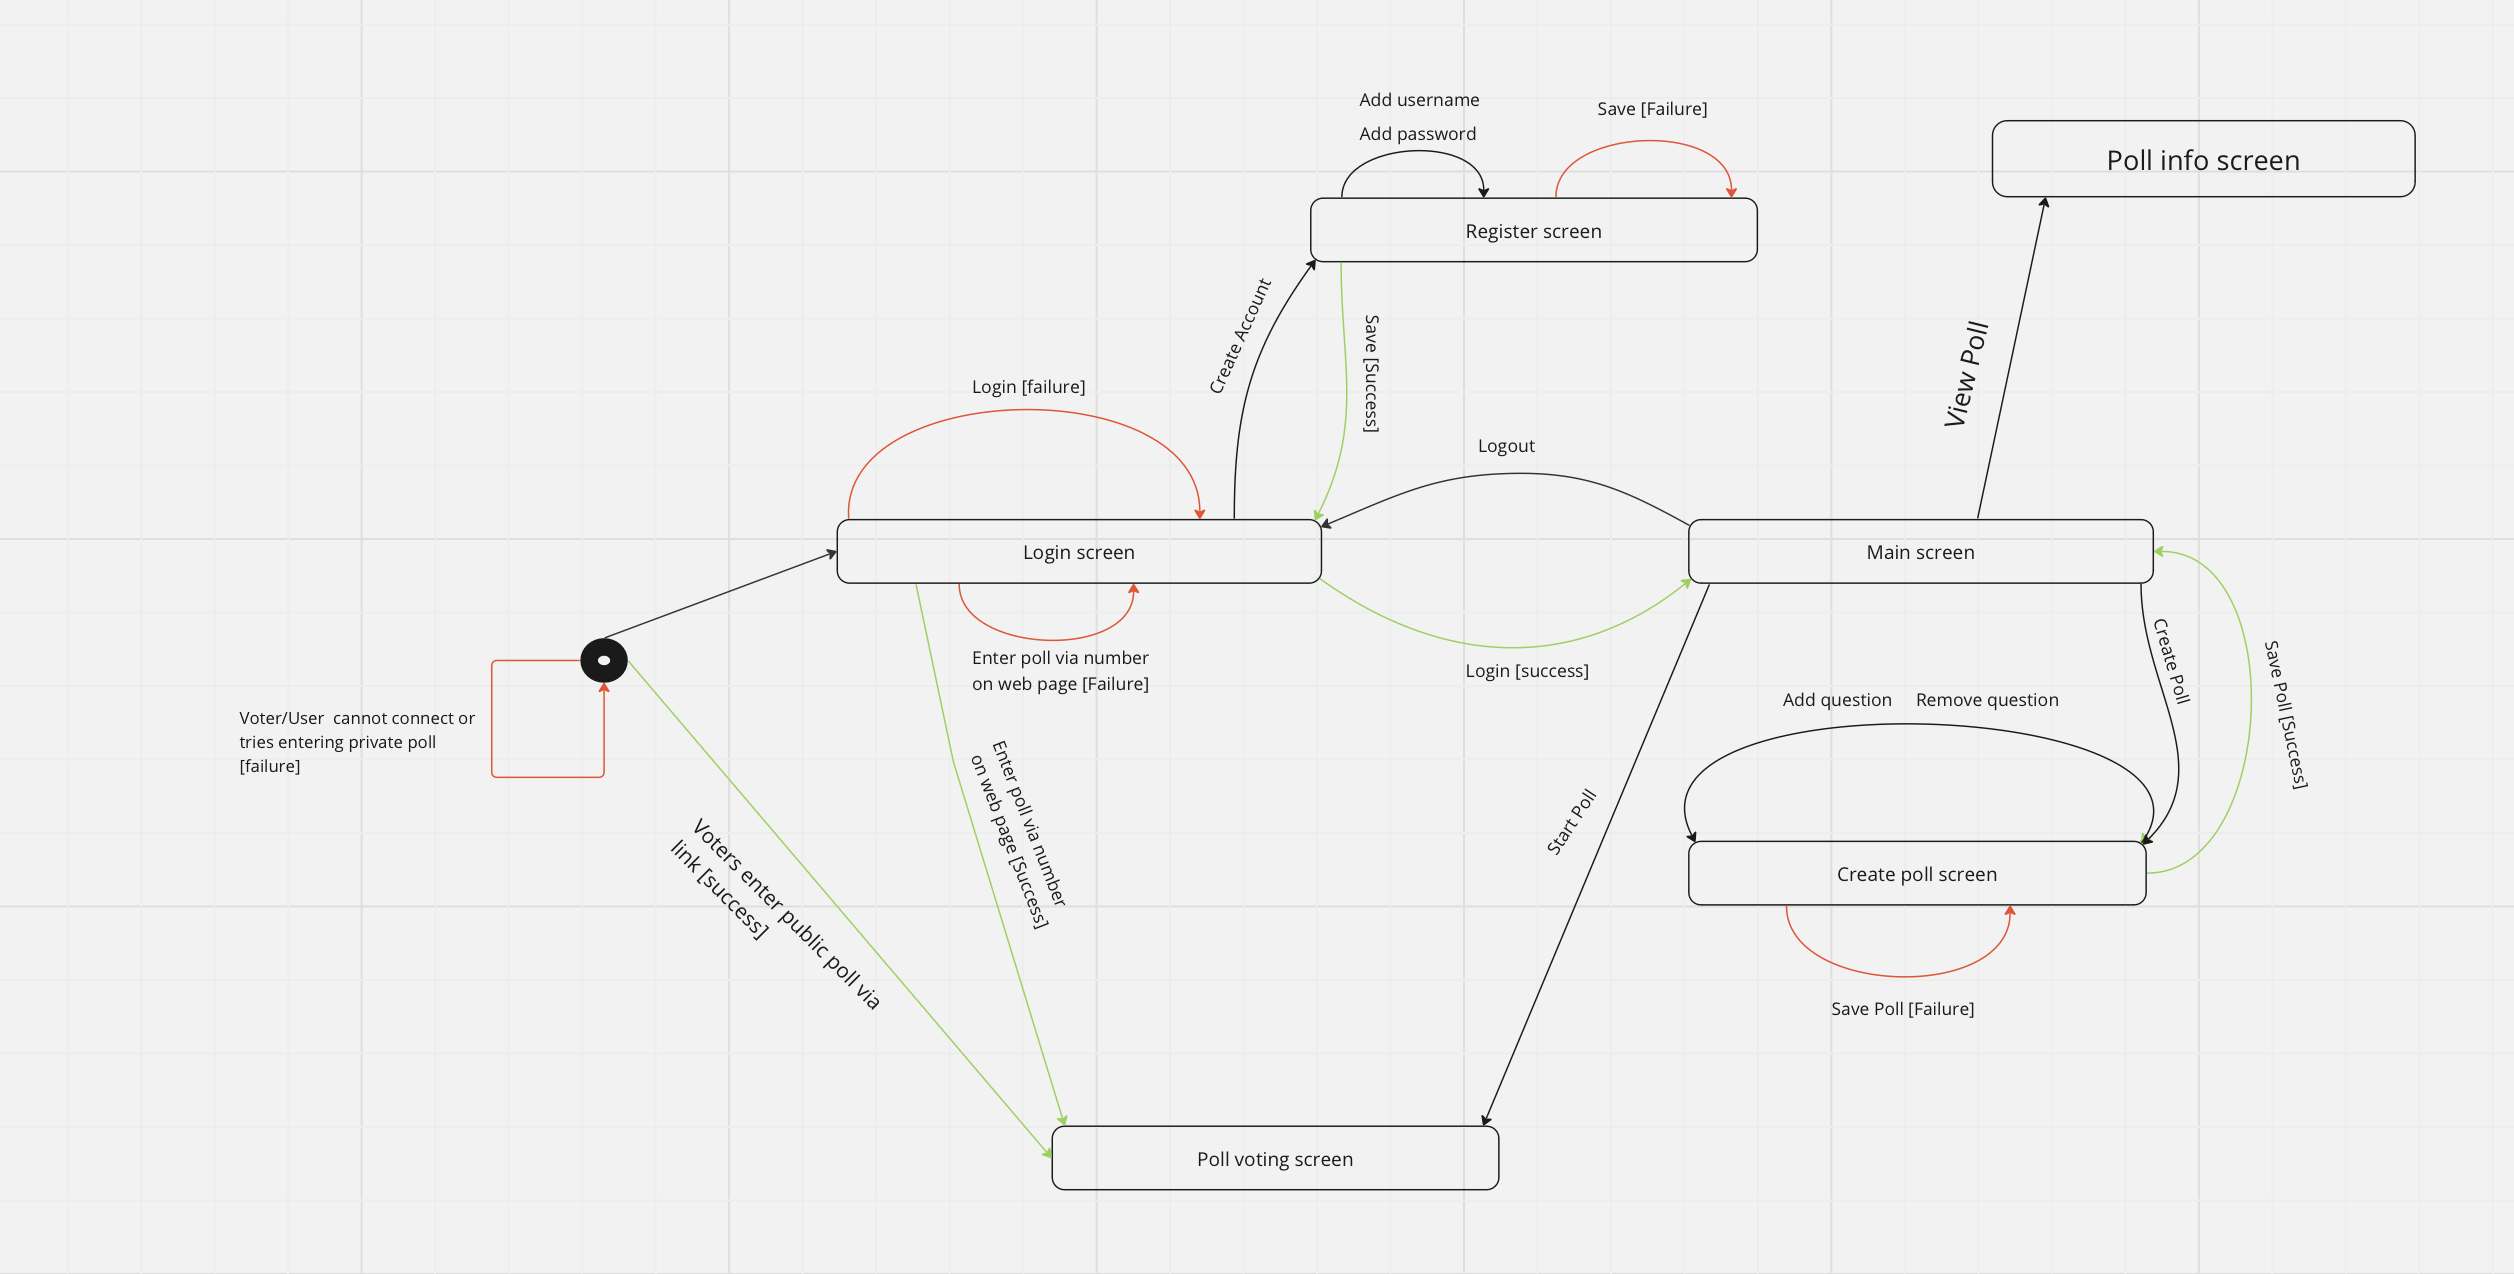
\includegraphics[scale=0.4]{figs/ApplicationFlowDiagram.png}



About 4 pages on:

\begin{enumerate}

\item An architectural overview of the application that has been implemented
\item High-level design, domain model, … (App assignment A)
\item May involve selected models from Chaps. 5 of the IoT and cloud books


\end{enumerate}

The example below shows how you may include code. There are similar
styles for many other langages - in case you do not use Java in your
project. You can wrap the listing into a figure in case you need to
refer to it. How to create a figure was shown in Section~\ref{sec:technology}.

\lstinputlisting[language=java]{code/BoksVolum.java}
